\begin{figure}[htbp]\centering
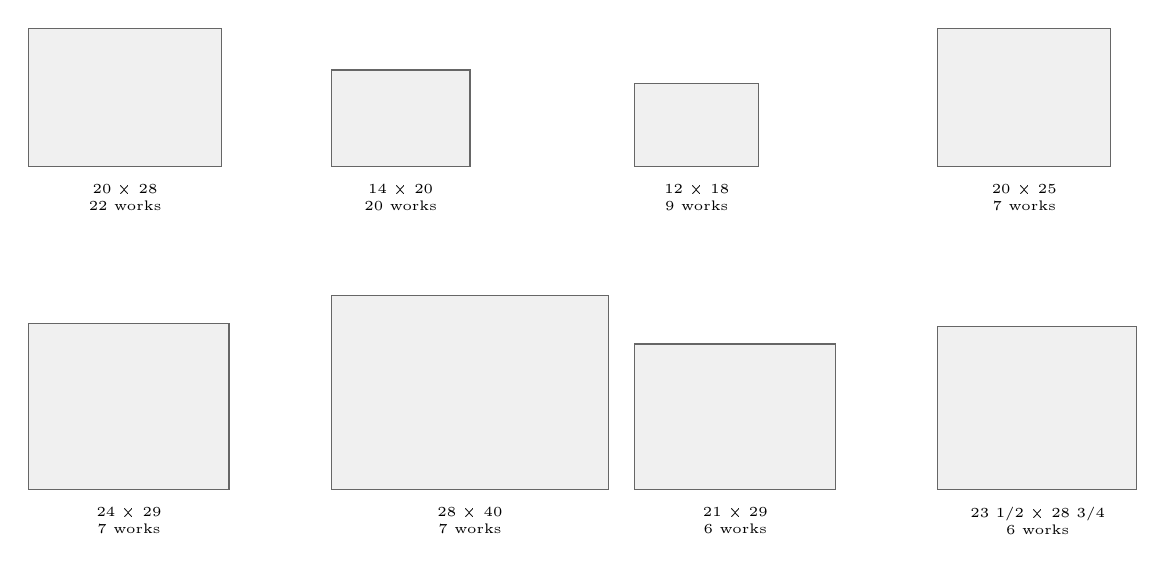
\begin{tikzpicture}
\draw[fill=black!6,draw=black!60] (0.00,0.00) rectangle (2.46,1.76);
\node[anchor=north,font=\tiny,align=center] at (1.23,-0.10) {20 × 28\\22 works};
\draw[fill=black!6,draw=black!60] (3.85,0.00) rectangle (5.61,1.23);
\node[anchor=north,font=\tiny,align=center] at (4.73,-0.10) {14 × 20\\20 works};
\draw[fill=black!6,draw=black!60] (7.70,0.00) rectangle (9.28,1.06);
\node[anchor=north,font=\tiny,align=center] at (8.49,-0.10) {12 × 18\\9 works};
\draw[fill=black!6,draw=black!60] (11.55,0.00) rectangle (13.75,1.76);
\node[anchor=north,font=\tiny,align=center] at (12.65,-0.10) {20 × 25\\7 works};
\draw[fill=black!6,draw=black!60] (0.00,-4.10) rectangle (2.55,-1.99);
\node[anchor=north,font=\tiny,align=center] at (1.28,-4.20) {24 × 29\\7 works};
\draw[fill=black!6,draw=black!60] (3.85,-4.10) rectangle (7.37,-1.64);
\node[anchor=north,font=\tiny,align=center] at (5.61,-4.20) {28 × 40\\7 works};
\draw[fill=black!6,draw=black!60] (7.70,-4.10) rectangle (10.25,-2.25);
\node[anchor=north,font=\tiny,align=center] at (8.98,-4.20) {21 × 29\\6 works};
\draw[fill=black!6,draw=black!60] (11.55,-4.10) rectangle (14.08,-2.03);
\node[anchor=north,font=\tiny,align=center] at (12.82,-4.20) {23 1/2 × 28 3/4\\6 works};
\end{tikzpicture}
\caption{The eight formats he came back to, drawn to one scale and to their real proportions, so that a watercolour half-sheet stands beside a five-foot canvas; each is labelled with the number of work headings read at that size. After the Technique tab. Drawn by Claude Fable~5.1, 13 September 2026, from \texttt{formats.json} (undated).}\label{fig:eight}
\end{figure}
